\documentclass[10pt,letterpaper, cm]{hmcpset}
\usepackage[top=0.5in,bottom=1in,right=1in,left=0.75in]{geometry}
\usepackage{multicol,graphicx, enumerate, cancel, amsmath, amsthm}
\usepackage{tikz}
\usepackage{tikz,fullpage}

\usetikzlibrary{arrows,petri,topaths}
				
\usepackage{tkz-berge}
\usepackage{tkz-graph}

\name{Jonathon Sonesen}
\class{CS 251}
\duedate{\today}
\assignment{Graph Theory Knowledge}
\extraline{Collaborators:Jeff Patterson, Steven Wetherebee, Kyle Kneitenger}

\setlength{\columnsep}{0.5cm}
\setlength{\columnseprule}{00pt}
\begin{document}


\section*{Graph Theory Knowledge Assignment}

\begin{problem}[1]

  Let $G$ be a simple graph with $n$ nodes. 
  Let $k$ be the number of edges of $G$. Prove (or disprove)
  \[k \leq \frac{n(n-1)}{2}\]
\end{problem}

\begin{array}{lll}
Row & Statement & Comment \\
1.  & Let~n:=1 &\text{Base~case}\\
2.  & G_1~has~0~edges~and~\frac{1(1-1)}{2}=0 &\text{by~example~10.1.9,and~subs.}\\
3.  & k \leq \frac{n(n-1)}{2} & \text{inductive~hyp.}\\
4.  & k = \frac{n(n-1)}{2}=\frac{(n+1)((n+1)-1)}{2}&\\
5.  & =\frac{n(n+1)}{2} + n &\\
6.  & =\frac{n(n+1)}{2} + \frac{2n}{2}&\\
7.  & =\frac{n^2-n+2n}{2} &\\
8.  & =\frac{n(n+1)}{2}&\\
9.  & \therefore k \leq \frac{n(n-1)}{2} &\text{QED}\\ 
\end{array}
\\
\begin{problem}[2]

  Let $G$ be the graph:

  \begin{center}
      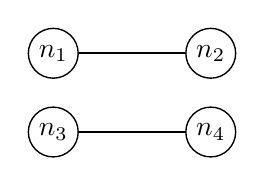
\begin{tikzpicture}[scale=1,transform shape]
        \GraphInit[vstyle=Dijkstra]
        \SetVertexMath

        \Vertex[x=0,y=0]{n_1}
        \Vertex[x=2,y=0]{n_2}
        \Vertex[x=0,y=-1]{n_3}
        \Vertex[x=2,y=-1]{n_4}
        \Edge[](n_1)(n_2)
        \Edge[](n_3)(n_4)
    \end{tikzpicture}
  \end{center}
What is the complement of $G$?
\end{problem}

  \begin{center}
      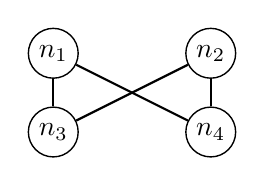
\begin{tikzpicture}[scale=1,transform shape]
        \GraphInit[vstyle=Dijkstra]
        \SetVertexMath

        \Vertex[x=0,y=0]{n_1}
        \Vertex[x=2,y=0]{n_2}
        \Vertex[x=0,y=-1]{n_3}
        \Vertex[x=2,y=-1]{n_4}
        \Edge[](n_1)(n_4)
        \Edge[](n_3)(n_2)
        \Edge[](n_1)(n_3)
        \Edge[](n_2)(n_4)
    \end{tikzpicture}
  \end{center}

\begin{problem}[3]
  List a simple graph that has 4 nodes of different degrees, or prove that no such graph exists.
\end{problem}\\
\\The proof to question 1 proves a contradiction\\\\
\begin{problem}[4]
What is the maximum number of edges possible in a disconnected graph with $n$ nodes and no loops or parallel edges?  Explain your answer. (No proof needed)
\end{problem}
k_{max}=\frac{n(n-1)}{2}\\

\begin{problem}[5]
Let $G$ be the graph:


\begin{center}

    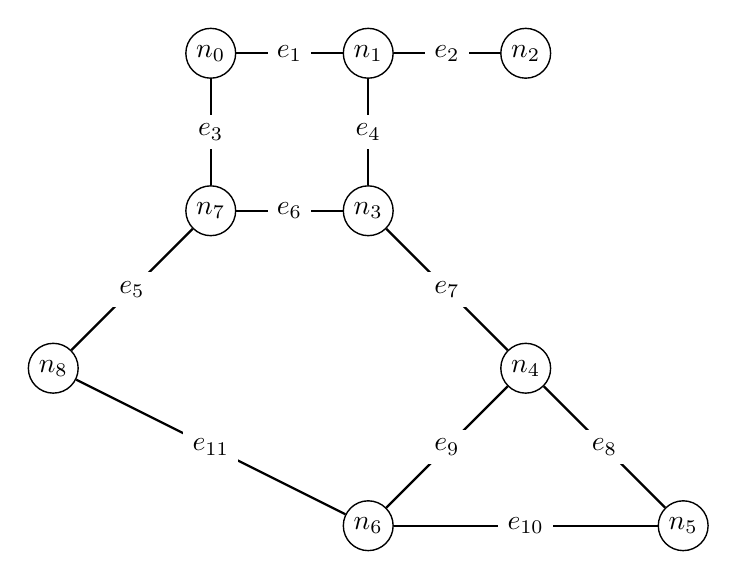
\begin{tikzpicture}[scale=1,transform shape]

        \GraphInit[vstyle=Dijkstra]

        \SetVertexMath
        \Vertex[x=0, y=0]{n_0}
        \Vertex[x=2, y=0]{n_1}
        \Vertex[x=4, y=0]{n_2}
        \Vertex[x=2, y=-2]{n_3}
        \Vertex[x=4, y=-4]{n_4}
        \Vertex[x=6, y=-6]{n_5}
        \Vertex[x=2, y=-6]{n_6}
        \Vertex[x=0, y=-2]{n_7}
        \Vertex[x=-2, y=-4]{n_8}
        \Edge[label=$e_1$](n_0)(n_1)
        \Edge[label=$e_2$](n_1)(n_2)
        \Edge[label=$e_3$](n_0)(n_7)
        \Edge[label=$e_4$](n_1)(n_3)
        \Edge[label=$e_5$](n_7)(n_8)
        \Edge[label=$e_6$](n_7)(n_3)
        \Edge[label=$e_7$](n_3)(n_4)
        \Edge[label=$e_8$](n_4)(n_5)
        \Edge[label=$e_9$](n_4)(n_6)
        \Edge[label=$e_{10}$](n_6)(n_5)
        \Edge[label=$e_{11}$](n_6)(n_8)
    \end{tikzpicture}
\end{center}

\begin{enumerate}[(a)]
    \item List the Adjacency matrix for this graph
    \item List the Incidence matrix for this graph
\end{enumerate}
\end{problem}



\begin{enumerate}[(a)]
    \item 
    
    \begin{align*}

      AM_G &= \begin{pmatrix}


         n_i & 0 & 1 & 2 & 3 & 4 & 5 & 6 & 7 & 8 \\        

         0   & 0 & 1 & 0 & 0 & 0 & 0 & 0 & 1 & 0 \\

         1   & 1 & 0 & 1 & 1 & 0 & 0 & 0 & 0 & 0 \\

         2   & 0 & 1 & 0 & 0 & 0 & 0 & 0 & 0 & 0 \\

         3   & 0 & 1 & 0 & 0 & 1 & 0 & 0 & 1 & 0  \\

         4   & 0 & 0 & 0 & 1 & 0 & 1 & 1 & 0 & 0 \\

         5   & 0 & 0 & 0 & 0 & 1 & 0 & 1 & 0 & 0 \\

         6   & 0 & 0 & 0 & 0 & 1 & 1 & 0 & 0 & 0 \\

         7   & 1 & 0 & 0 & 1 & 0 & 0 & 0 & 0 & 1 \\

         8   & 0 & 0 & 0 & 0 & 0 & 0 & 0 & 1 & 0

      \end{pmatrix}  
              \end{align*}

    \item 
      \begin{align*}
      
      \setcounter{MaxMatrixCols}{20}
     LM_G&=
      \begin{pmatrix}


             1 & 1 & 0 & 0 & 0 & 0 & 0 & 0 & 0 & 0 & 0\\        

             1 & 0 & 1 & 1 & 0 & 0 & 0 & 0 & 0 & 0 & 0\\ 

             0 & 0 & 1 & 0 & 0 & 0 & 0 & 0 & 0 & 0 & 0\\

             0 & 1 & 0 & 0 & 1 & 1 & 0 & 0 & 0 & 0 & 0\\

             0 & 0 & 0 & 1 & 1 & 0 & 1 & 0 & 0 & 0 & 0\\

             0 & 0 & 0 & 0 & 0 & 1 & 0 & 1 & 0 & 0 & 0\\

             0 & 0 & 0 & 0 & 0 & 0 & 1 & 0 & 1 & 1 & 0\\

             0 & 0 & 0 & 0 & 0 & 0 & 0 & 0 & 1 & 0 & 1\\

             0 & 0 & 0 & 0 & 0 & 0 & 0 & 1 & 0 & 1 & 1

         \end{pmatrix}  
      \end{align*}
      \end{enumerate}

    \begin{problem}[6]
    Let $G$ be the graph:

    \begin{center}
    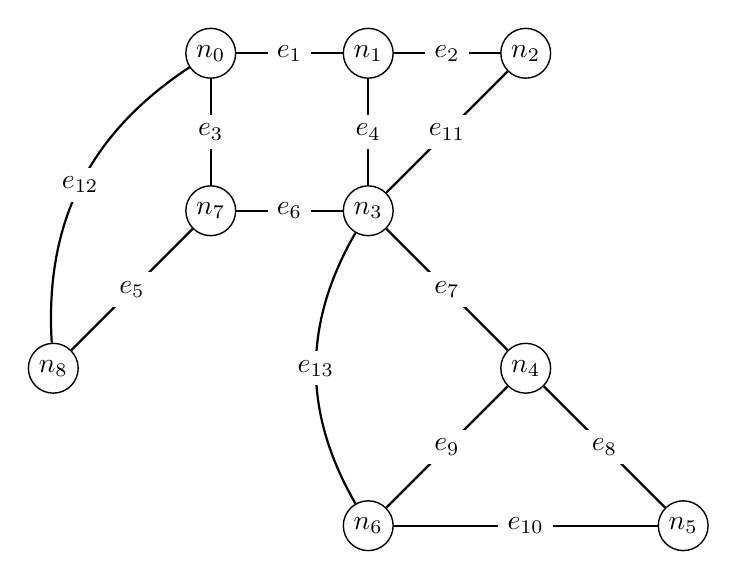
\begin{tikzpicture}[scale=1,transform shape]
        \GraphInit[vstyle=Dijkstra]
        \SetVertexMath

        \Vertex[x=0, y=0]{n_0}
        \Vertex[x=2, y=0]{n_1}
        \Vertex[x=4, y=0]{n_2}
        \Vertex[x=2, y=-2]{n_3}
        \Vertex[x=4, y=-4]{n_4}
        \Vertex[x=6, y=-6]{n_5}
        \Vertex[x=2, y=-6]{n_6}
        \Vertex[x=0, y=-2]{n_7}
        \Vertex[x=-2, y=-4]{n_8}
        \Edge[label=$e_1$](n_0)(n_1)
        \Edge[label=$e_2$](n_1)(n_2)
        \Edge[label=$e_3$](n_0)(n_7)
        \Edge[label=$e_4$](n_1)(n_3)
        \Edge[label=$e_5$](n_7)(n_8)
        \Edge[label=$e_6$](n_7)(n_3)
        \Edge[label=$e_7$](n_3)(n_4)
        \Edge[label=$e_8$](n_4)(n_5)
        \Edge[label=$e_9$](n_4)(n_6)
        \Edge[label=$e_{10}$](n_6)(n_5)
        \Edge[label=$e_{11}$](n_3)(n_2)
        \Edge[style={bend right}, label= $e_{12}$](n_0)(n_8)
        \Edge[style={bend right}, label= $e_{13}$](n_3)(n_6)

    \end{tikzpicture}
    \end{center}

    \begin{enumerate}[(a)]
        \item List the Laplacian matrix for this graph
        \item List the eigenvalues for the Laplacian matrix for this graph
    \end{enumerate}
\end{problem}

\begin{enumerate}[(a)]

    \item 
    
    \begin{align*}

      LM_G &= \begin{pmatrix}



           & 3 & -1 & 0 & 0 & 0 & 0 & 0 & -1 & -1 \\

           & -1 & 3 & -1 & -1 & 0 & 0 & 0 & 0 & 0 \\

           & 0 & -1 & 2 & -1 & 0 & 0 & 0 & 0 & 0 \\

           & 0 & -1 & -1 & 5 & -1 & 0 & -1 & -1 & 0  \\

           & 0 & 0 & 0 & -1 & 3 & -1 & -1 & 0 & 0 \\

           & 0 & 0 & 0 & 0 & -1 & 2 & -1 & 0 & 0 \\

           & 0 & 0 & 0 & -1 & -1 & -1 & 3 & 0 & 0 \\

           & -1 & 0 & 0 & -1 & 0 & 0 & 0 & 3 & -1 \\

           & -1 & 0 & 0 & 0 & 0 & 0 & 0 & -1 & 2

      \end{pmatrix}  
              \end{align*}

  \item
    \begin{align*}
      EV_{LM} & = \begin{bmatrix}
        6.3586\\
        4.3977\\
        4.0000\\
        3.5651\\
        3.0000\\
        3.0000\\
        1.1760\\
        0.5126\\
        0.0000\\
      \end{bmatrix}
    \end{align*}
\end{enumerate}


\begin{problem}[7]
    Let $G$ be the graph:

    \begin{center}
    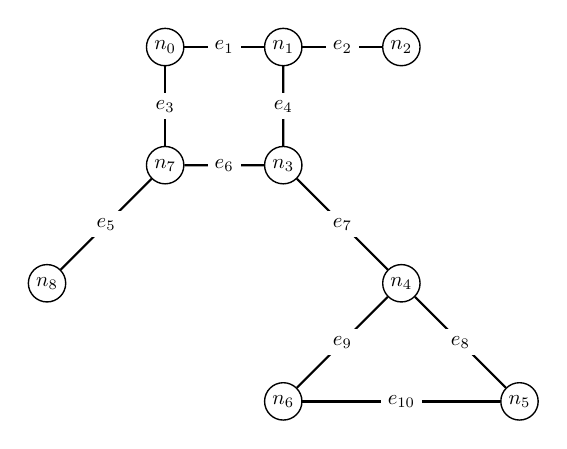
\begin{tikzpicture}[scale=.75, transform shape]
        \GraphInit[vstyle=Dijkstra]
        \SetVertexMath

        \Vertex[x=0, y=0]{n_0}
        \Vertex[x=2, y=0]{n_1}
        \Vertex[x=4, y=0]{n_2}
        \Vertex[x=2, y=-2]{n_3}
        \Vertex[x=4, y=-4]{n_4}
        \Vertex[x=6, y=-6]{n_5}
        \Vertex[x=2, y=-6]{n_6}
        \Vertex[x=0, y=-2]{n_7}
        \Vertex[x=-2, y=-4]{n_8}
        \Edge[label=$e_1$](n_0)(n_1)
        \Edge[label=$e_2$](n_1)(n_2)
        \Edge[label=$e_3$](n_0)(n_7)
        \Edge[label=$e_4$](n_1)(n_3)
        \Edge[label=$e_5$](n_7)(n_8)
        \Edge[label=$e_6$](n_7)(n_3)
        \Edge[label=$e_7$](n_3)(n_4)
        \Edge[label=$e_8$](n_4)(n_5)
        \Edge[label=$e_9$](n_4)(n_6)
        \Edge[label=$e_{10}$](n_6)(n_5)

    \end{tikzpicture}
    \end{center}

    \begin{enumerate}[(a)]
        \item List the Degree matrix for this graph
        \item List the Adjacency matrix for this graph
        \item Identify the bridges (if any) of this graph. If ther are no bridges, write ``none''.
    \end{enumerate}
\end{problem}

\begin{enumerate}[(a)]

    \item 
    
    \begin{align*}

      DM_G &= \begin{pmatrix}


         n_i & 0 & 1 & 2 & 3 & 4 & 5 & 6 & 7 & 8 \\        

         0   & 2 & 0 & 0 & 0 & 0 & 0 & 0 & 0 & 0 \\

         1   & 0 & 3 & 0 & 0 & 0 & 0 & 0 & 0 & 0 \\

         2   & 0 & 0 & 1 & 0 & 0 & 0 & 0 & 0 & 0 \\

         3   & 0 & 0 & 0 & 3 & 0 & 0 & 0 & 0 & 0  \\

         4   & 0 & 0 & 0 & 0 & 3 & 0 & 0 & 0 & 0 \\

         5   & 0 & 0 & 0 & 0 & 0 & 2 & 0 & 0 & 0 \\

         6   & 0 & 0 & 0 & 0 & 0 & 0 & 2 & 0 & 0 \\

         7   & 0 & 0 & 0 & 0 & 0 & 0 & 0 & 3 & 0 \\

         8   & 0 & 0 & 0 & 0 & 0 & 0 & 0 & 0 & 1

      \end{pmatrix}  
              \end{align*}
    \item 
    
    \begin{align*}

      DM_G &= \begin{pmatrix}


         n_i & 0 & 1 & 2 & 3 & 4 & 5 & 6 & 7 & 8 \\        

         0   & 0 & 1 & 0 & 0 & 0 & 0 & 0 & 0 & 0 \\

         1   & 1 & 1 & 1 & 0 & 0 & 0 & 0 & 0 & 0 \\

         2   & 0 & 1 & 0 & 0 & 0 & 0 & 0 & 0 & 0 \\

         3   & 0 & 1 & 0 & 0 & 1 & 0 & 0 & 1 & 0  \\

         4   & 0 & 0 & 0 & 1 & 0 & 1 & 1 & 0 & 0 \\

         5   & 0 & 0 & 0 & 0 & 1 & 0 & 1 & 0 & 0 \\

         6   & 0 & 0 & 0 & 0 & 1 & 1 & 0 & 0 & 0 \\

         7   & 1 & 0 & 0 & 1 & 0 & 0 & 0 & 0 & 0 \\

         8   & 0 & 0 & 0 & 0 & 0 & 0 & 0 & 1 & 0

      \end{pmatrix}  
              \end{align*}

  \item
    \begin{equation*}
      bridges:~\left\{e_2,e_5,e_7\right\}
    \end{equation*}
\end{enumerate}

\begin{problem}[8]
    Let $G$ be the graph:
    
    \begin{center}
    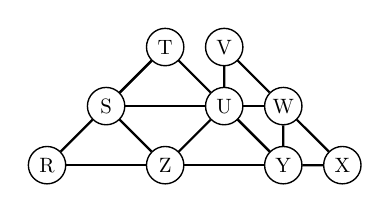
\begin{tikzpicture}[scale=.75, transform shape]
        \GraphInit[vstyle=Dijkstra]
        \SetGraphUnit{1}

        \Vertex{T} \EA(T){V}
        \SOWE(T){S} \SOEA(T){U} \SOEA(V){W}
        \SOWE(S){R} \SOWE(U){Z} \SOEA(U){Y} \SOEA(W){X}
        \Edges(T,S,R,Z,S,U,Z,Y,U,S,T,U,Y,X,W,Y,U,W,V,U)

    \end{tikzpicture}
    \end{center}

    \begin{enumerate}[(a)]
        \item List the Laplacian matrix for this graph
        \item List the Incidence matrix for this graph
        \item Identify an Euler circuit for this graph, or prove no such circuit exists
    \end{enumerate}
\end{problem}

\begin{enumerate}[(a)]

    \item 
    
    \begin{align*}

      LM_G &= \begin{pmatrix}


             & R & S & T & U & V & W & X & Y & Z \\        

         R   & 2 & -1 & 0 & 0 & 0 & 0 & 0 & 0 & -1 \\

         S   & -1 & 4 & -1 & -1 & 0 & 0 & 0 & 0 & -1 \\

         T   & 0 & -1 & 2 & -1 & 0 & 0 & 0 & 0 & 0 \\

         U   & 0 & -1 & -1 & 6 & -1 & -1 & 0 & -1 & -1  \\

         V   & 0 & 0 & 0 & -1 & 2 & -1 & 0 & 0 & 0 \\

         W   & 0 & 0 & 0 & -1 & -1 & 4 & -1 & -1 & 0 \\

         X   & 0 & 0 & 0 & 0 & 0 & -1 & 2 & -1 & 0 \\

         Y   & 0 & 0 & 0 & -1 & 0 & -1 & -1 & 4 & -1 \\

         Z   & -1 & -1 & 0 & -1 & 0 & 0 & 0 & -1 & 4

      \end{pmatrix}  
              \end{align*}
    \item 
    
    \begin{align*}
  
      IM_G &= \begin{pmatrix}


             & R & R & S & S & S & T & U & U & U & U & V & W & W & X & Y\\        

             & S & Z & T & U & Z & U & V & W & Y & Z & W & X & Y & Y & Z \\

         R   & 1 & 1 & 0 & 0 & 0 & 0 & 0 & 0 & 0 & 0 & 0 & 0 & 0 & 0 & 0\\

         S   & 1 & 0 & 1 & 1 & 1 & 0 & 0 & 0 & 0 & 0 & 0 & 0 & 0 & 0 & 0 \\

         T   & 0 & 0 & 1 & 0 & 0 & 1 & 0 & 1 & 0 & 0 & 0 & 0 & 0 & 0 & 0  \\

         U   & 0 & 0 & 0 & 1 & 0 & 1 & 1 & 1 & 1 & 1 & 0 & 0 & 0 & 0 & 0 \\

         V   & 0 & 0 & 0 & 0 & 0 & 0 & 1 & 0 & 0 & 0 & 1 & 0 & 0 & 0 & 0 \\

         W   & 0 & 0 & 0 & 0 & 0 & 0 & 0 & 1 & 0 & 0 & 1 & 1 & 1 & 0 & 0 \\

         X   & 1 & 0 & 0 & 1 & 0 & 0 & 0 & 0 & 0 & 0 & 0 & 1 & 0 & 1 & 0 \\

         Y   & 0 & 0 & 0 & 0 & 0 & 0 & 0 & 0 & 1 & 0 & 0 & 0 & 1 & 1 & 1 \\
         
         Z   & 0 & 1 & 0 & 0 & 1 & 0 & 0 & 0 & 0 & 0 & 0 & 0 & 0 & 1 & 1

      \end{pmatrix}  
              \end{align*}

  \item
    \begin{equation*}
      euler~circuit:~\left\{T, U, Y, X, W, Y, Z, R, S, Z, U, W, V, U, S, T\right\}
    \end{equation*}
\end{enumerate}

\begin{problem}[9]
    Let $G$ be the graph:
    \begin{center}
    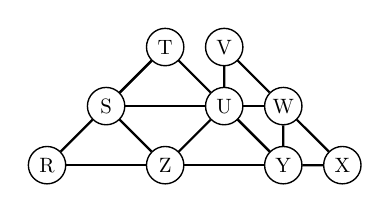
\begin{tikzpicture}[scale=.75, transform shape]
        \GraphInit[vstyle=Dijkstra]
        \SetGraphUnit{1}

        \Vertex{T} \EA(T){V}
        \SOWE(T){S} \SOEA(T){U} \SOEA(V){W}
        \SOWE(S){R} \SOWE(U){Z} \SOEA(U){Y} \SOEA(W){X}
        \Edges(T,S,R,Z,S,U,Z,Y,U,S,T,U,Y,X,W,Y,U,W,V,U)

    \end{tikzpicture}
    \end{center}

    \begin{enumerate}[(a)]
        \item List the Adjacency matrix for this graph
        \item List the Degree matrix for this graph
        \item Identify a Hamiltonian circuit for this graph, or prove no such circuit exists
    \end{enumerate}
\end{problem}

\begin{enumerate}[(a)]

    \item 
    
    \begin{align*}

      AM_G &= \begin{pmatrix}


             & R & S & T & U & V & W & X & Y & Z \\        

         R   & 0 & 1 & 0 & 0 & 0 & 0 & 0 & 0 & 1 \\

         S   & 1 & 0 & 1 & 0 & 0 & 0 & 0 & 0 & 1 \\

         T   & 0 & 1 & 0 & 1 & 0 & 0 & 0 & 0 & 0 \\

         U   & 0 & 1 & 1 & 0 & 1 & 1 & 0 & 1 & 1  \\

         V   & 0 & 0 & 0 & 1 & 0 & 1 & 0 & 0 & 0 \\

         W   & 0 & 0 & 0 & 1 & 1 & 0 & 1 & 1 & 0 \\

         X   & 0 & 0 & 0 & 0 & 0 & 1 & 0 & 1 & 0 \\

         Y   & 0 & 0 & 0 & 1 & 0 & 1 & 1 & 0 & 1 \\

         Z   & 1 & 1 & 0 & 1 & 0 & 0 & 0 & 1 & 0

      \end{pmatrix}  
              \end{align*}
    \item 
    
    \begin{align*}

      AM_G &= \begin{pmatrix}


             & R & S & T & U & V & W & X & Y & Z \\        

         R   & 2 & 0 & 0 & 0 & 0 & 0 & 0 & 0 & 0 \\

         S   & 0 & 4 & 0 & 0 & 0 & 0 & 0 & 0 & 0 \\

         T   & 0 & 0 & 2 & 0 & 0 & 0 & 0 & 0 & 0 \\

         U   & 0 & 0 & 0 & 6 & 0 & 0 & 0 & 0 & 0  \\

         V   & 0 & 0 & 0 & 0 & 2 & 0 & 0 & 0 & 0 \\

         W   & 0 & 0 & 0 & 0 & 0 & 4 & 0 & 0 & 0 \\

         X   & 0 & 0 & 0 & 0 & 0 & 0 & 2 & 0 & 0 \\

         Y   & 0 & 0 & 0 & 0 & 0 & 0 & 0 & 0 & 0 \\

         Z   & 0 & 0 & 0 & 0 & 0 & 0 & 0 & 0 & 4

      \end{pmatrix}  
              \end{align*}

  \item
    \begin{equation*}
      hamiltonian~circuit:~\left\{T, S, R, Z, Y, Y, X, W, V, U, T\right\}
    \end{equation*}
\end{enumerate}
\begin{problem}[10]
    Let $G$ be the graph:
    \begin{center}
    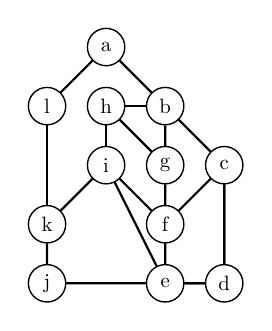
\begin{tikzpicture}[scale=.75, transform shape]
        \GraphInit[vstyle=Dijkstra]
        \SetGraphUnit{1}

        \Vertex{a} \SOWE(a){l} \SO(a){h} \SOEA(a){b}
	\SO(h){i} \SO(b){g} \SOEA(b){c}
	\SOWE(i){k} \SOEA(i){f}
	\SO(k){j} \SO(f){e} \SOEA(f){d}
        \Edges(a,l,k,j,e,d,c,b,a)
        \Edges(k,i,h,b,g,h,i,f,c,d,e,i)
        \Edges(e,f,g)
    \end{tikzpicture}
    \end{center}

    \begin{enumerate}[(a)]
        \item List the Adjacency matrix for this graph
        \item List the Degree matrix for this graph
        \item Identify an Euler circuit for this graph, or prove no such circuit exists
    \end{enumerate}
\end{problem}

\begin{enumerate}[(a)]

    \item 
    
    \begin{align*}

      AM_G &= \begin{pmatrix}


             & A & B & C & D & E & F & G & H & I & J & K & L \\        

         A   & 0 & 1 & 0 & 0 & 0 & 0 & 0 & 0 & 0 & 0 & 0 & 1 \\

         B   & 1 & 0 & 1 & 0 & 0 & 0 & 1 & 1 & 0 & 0 & 0 & 0\\

         C   & 0 & 1 & 0 & 1 & 0 & 1 & 0 & 0 & 0  & 0 & 0 & 0\\

         D   & 0 & 0 & 1 & 0 & 1 & 0 & 0 & 0 & 0  & 0 & 0 & 0 \\

         E   & 0 & 0 & 0 & 1 & 0 & 1 & 0 & 0 & 1 & 1 & 0 & 0\\

         F   & 0 & 0 & 1 & 0 & 1 & 0 & 1 & 0 & 1 & 0 & 0 & 0 \\

         G   & 0 & 1 & 0 & 0 & 0 & 1 & 0 & 1 & 0 & 0 & 0 & 0\\

         H   & 0 & 1 & 0 & 0 & 0 & 0 & 1 & 0 & 1 & 0 & 0 & 0\\

         I   & 0 & 0 & 0 & 0 & 1 & 1 & 0 & 1 & 0 & 0 & 1 & 0\\
          
         J   & 0 & 0 & 0 & 0 & 1 & 0 & 0 & 0 & 0 & 0 & 1 & 0 \\

         K   & 0 & 0 & 0 & 0 & 0 & 0 & 0 & 0 & 1 & 1 & 0 & 1 \\

         L   & 1 & 0 & 0 & 0 & 0 & 0 & 0 & 0 & 0 & 0 & 1 & 0
      \end{pmatrix}  
              \end{align*}
    \item 
    
    \begin{align*}

      AM_G &= \begin{pmatrix}


             & A & B & C & D & E & F & G & H & I & J & K & L \\        

         A   & 2 & 0 & 0 & 0 & 0 & 0 & 0 & 0 & 0 & 0 & 0 & 0 \\

         B   & 0 & 4 & 0 & 0 & 0 & 0 & 0 & 0 & 0 & 0 & 0 & 0\\

         C   & 0 & 0 & 3 & 0 & 0 & 0 & 0 & 0 & 0  & 0 & 0 & 0\\

         D   & 0 & 0 & 0 & 2 & 0 & 0 & 0 & 0 & 0  & 0 & 0 & 0 \\

         E   & 0 & 0 & 0 & 0 & 4 & 0 & 0 & 0 & 0 & 0 & 0 & 0\\

         F   & 0 & 0 & 0 & 0 & 0 & 4 & 0 & 0 & 0 & 0 & 0 & 0 \\

         G   & 0 & 0 & 0 & 0 & 0 & 0 & 3 & 0 & 0 & 0 & 0 & 0\\

         H   & 0 & 0 & 0 & 0 & 0 & 0 & 0 & 3 & 0 & 0 & 0 & 0\\

         I   & 0 & 0 & 0 & 0 & 0 & 0 & 0 & 0 & 4 & 0 & 0 & 0\\
          
         J   & 0 & 0 & 0 & 0 & 0 & 0 & 0 & 0 & 0 & 2 & 0 & 0 \\

         K   & 0 & 0 & 0 & 0 & 0 & 0 & 0 & 0 & 0 & 0 & 3 & 0 \\

         L   & 0 & 0 & 0 & 0 & 0 & 0 & 0 & 0 & 0 & 0 & 0 & 2
      \end{pmatrix}  
              \end{align*}
  \item
    By the contrapositive version of theorem 10.2.2 in the epp text:\\
    If some vertex of a graph has odd degree, then the graph does not have an euler circuit.
\end{enumerate}

\begin{problem}[11]
    Let $G$ be the graph:
    \begin{center}
    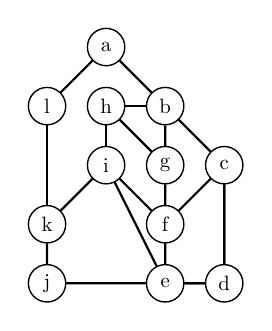
\begin{tikzpicture}[scale=.75, transform shape]
        \GraphInit[vstyle=Dijkstra]
        \SetGraphUnit{1}

        \Vertex{a} \SOWE(a){l} \SO(a){h} \SOEA(a){b}
	\SO(h){i} \SO(b){g} \SOEA(b){c}
	\SOWE(i){k} \SOEA(i){f}
        \SO(k){j} \SO(f){e} \SOEA(f){d}
        \Edges(a,l,k,j,e,d,c,b,a)
        \Edges(k,i,h,b,g,h,i,f,c,d,e,i)
        \Edges(e,f,g)

    \end{tikzpicture}
    \end{center}

    \begin{enumerate}[(a)]
        \item List the Laplacian matrix for this graph
        \item List the Incidence matrix for this graph
        \item Identify a Hamiltonian circuit for this graph, or prove no such circuit exists
        \end{enumerate}
\end{problem}

\begin{enumerate}[(a)]

    \item 
    
    \begin{align*}

      LM_G &= \begin{pmatrix}


             & A & B & C & D & E & F & G & H & I & J & K & L \\        

         A   & 2 & -1 & 0 & 0 & 0 & 0 & 0 & 0 & 0 & 0 & 0 & -1 \\

         B   & -1 & 4 & -1 & 0 & 0 & 0 & -1 & -1 & 0 & 0 & 0 & 0\\

         C   & 0 & -1 & 3 & -1 & 0 & -1 & 0 & 0 & 0  & 0 & 0 & 0\\

         D   & 0 & 0 & -1 & 2 & -1 & 0 & 0 & 0 & 0  & 0 & 0 & 0 \\

         E   & 0 & 0 & 0 & -1 & 4 & -1 & 0 & 0 & -1 & -1 & 0 & 0\\

         F   & 0 & 0 & -1 & 0 & -1 & 4 & -1 & 0 & -1 & 0 & 0 & 0 \\

         G   & 0 & -1 & 0 & 0 & 0 & -1 & 3 & -1 & 0 & 0 & 0 & 0\\

         H   & 0 & -1 & 0 & 0 & 0 & 0 & -1 & 3 & -1 & 0 & 0 & 0\\

         I   & 0 & 0 & 0 & 0 & -1 & -1 & 0 & -1 & 4 & 0 & -1 & 0\\
          
         J   & 0 & 0 & 0 & 0 & -1 & 0 & 0 & 0 & 0 & 2 & -1 & 0 \\

         K   & 0 & 0 & 0 & 0 & 0 & 0 & 0 & 0 & -1 & -1 & 3 & -1 \\

         L   & -1 & 0 & 0 & 0 & 0 & 0 & 0 & 0 & 0 & 0 & -1 & 2
      \end{pmatrix}  
              \end{align*}
    \item 
    
    \begin{align*}

      IM_G &= \begin{pmatrix}


             & A & A & B & B & B & C & C & D & E & E & E & F & F & G & H & I & J & K \\
             & B & L & C & G & H & D & F & E & F & I & J & G & I & H & I & K & K & L \\

         A   & 1 & 1 & 0 & 0 & 0 & 0 & 0 & 0 & 0 & 0 & 0 & 0 & 0 & 0 & 0 & 0 & 0 & 0  \\

         B   & 0 & 0 & 1 & 1 & 1 & 0 & 0 & 0 & 0 & 0 & 0 & 0 & 0 & 0 & 0 & 0 & 0 & 0\\

         C   & 0 & 0 & 1 & 0 & 0 & 1 & 1 & 0 & 0 & 0 & 0 & 0 & 0 & 0 & 0 & 0 & 0 & 0\\

         D   & 0 & 0 & 0 & 0 & 0 & 1 & 1 & 0 & 0 & 0 & 0 & 0 & 0 & 0 & 0 & 0 & 0 & 0 \\

         E   & 0 & 0 & 0 & 0 & 0 & 0 & 0 & 1 & 1 & 1 & 1 & 0 & 0 & 0 & 0 & 0 & 0 & 0\\

         F   & 0 & 0 & 0 & 0 & 0 & 0 & 1 & 1 & 0 & 0 & 1 & 1 & 1 & 0 & 0 & 0 & 0 & 0 \\

         G   & 0 & 0 & 0 & 0 & 0 & 0 & 0 & 0 & 0 & 0 & 0 & 0 & 0 & 0 & 0 & 0 & 0 & 0\\

         H   & 0 & 0 & 0 & 0 & 0 & 0 & 0 & 0 & 0 & 0 & 0 & 0 & 0 & 0 & 0 & 0 & 0 & 0\\

         I   & 0 & 0 & 0 & 0 & 0 & 0 & 0 & 0 & 0 & 1 & 0 & 0 & 1 & 0 & 1 & 1 & 0 & 0\\
          
         J   & 0 & 0 & 0 & 0 & 0 & 0 & 0 & 0 & 0 & 0 & 1 & 0 & 0 & 0 & 0 & 0 & 1 & 0 \\

         K   & 0 & 0 & 0 & 0 & 0 & 0 & 0 & 0 & 0 & 0 & 0 & 0 & 0 & 0 & 0 & 1 & 1 & 1 \\

         L   & 0 & 1 & 0 & 0 & 0 & 0 & 0 & 0 & 0 & 0 & 0 & 0 & 0 & 0 & 0 & 0 & 0 & 1
      \end{pmatrix}  
              \end{align*}
  \item
    \begin{equation*}
      Hamiltonian~circuit:\left\{b,a,l,k,j,e,d,c,f,i,h,g,b\right\}
    \end{equation*}
\end{enumerate}

\begin{problem}[12]

  
  Let
  \begin{center}

    M &=
    \begin{pmatrix}
      0 & 0\\
      0 & 0\\

    \end{pmatrix}
  \end{center}
 List two 2 x 2 matrices A and B that sitisfy *all* of the following conditions:\\
 \begin{enumerate}[-]
   \item $A\neq M$\\
   \item $B\neq M$\\
   \item $AB\neq M$\\
   \item $BA\neq M$\\
 \end{enumerate}  

\end{problem}

  \begin{center}

    A &=
    \begin{pmatrix}
      1 & 0\\
      0 & 0\\

    \end{pmatrix},
    B &=
    \begin{pmatrix}
      0 & 1\\
      0 & 0\\

    \end{pmatrix}

    A &=
    \begin{pmatrix}
      2 & 0\\
      0 & 0\\

    \end{pmatrix},
    B &=
    \begin{pmatrix}
      0 & 2\\
      0 & 0\\
    \end{pmatrix}
  \end{center}

  \begin{problem}
    Let
    \begin{align*}
      M = \begin{pmatrix}
        4 & 12 & 7 & 3 & 20 \\
        12 & 4 & 20 & 21 & 7  \\
        10 & 7 & 6 & 9 & 13 \\
        1 & 2 & 3 & 4 & 5 \\
        10 & 8 & 15 & 13 & 12
      \end{pmatrix}
    \end{align*}
    List the matrix m^6
  \end{problem}
    
  \begin{align*}
      M^6 = \begin{pmatrix}
        1574709790 &  1574709790 & 2106725231 & 2076398918 & 2415751821 \\
        1643310630 & 1463710842 & 2196967681 & 2166165175 & 2521712946  \\
        1366176423 & 1216993970 & 1826701919 & 1800937567 & 2096602872 \\
        1 & 2 & 3 & 4 & 5 \\
        10 & 8 & 15 & 13 & 12
      \end{pmatrix}
    \end{align*}
  
  \end{document}
